\documentclass[a4paper,12pt]{article} % Prepara un documento per carta A4, con un bel font grande

% impostazioni generali del documento, valide per tutti gli scritti.

\usepackage{graphicx} % per l'inserimento di immagini.
\usepackage{listings}
\lstloadlanguages{PROLOG}
\usepackage[italian]{babel} % Adatta LaTeX alle convenzioni tipografiche italiane,
% e ridefinisce alcuni titoli in italiano, come "Capitolo" al posto di "Chapter", se il vostro documento in italiano
\usepackage[utf8]{inputenc} % Consente l'uso caratteri accentati italiani


\usepackage{fancyhdr} % per il controllo delle intestazioni.
\usepackage{totpages} % macro per conoscere il tatale delle pagine
\usepackage{longtable} % tabelle che vanno su pi� pagine
\frenchspacing % forza LaTeX ad una spaziatura fra parole non inglesi

\pagestyle{fancy}

\newcommand{\linkref}[1]{{\footnotesize \textsl{#1}}}


% fine delle impostazioni generali

\newtoks\titolo % definisco un nuovo comando \titolo che restituisce il titolo.
\newtoks\versione % definisco un nuovo comando \versione che restituisce il versione.
\newtoks\data   % definisco un nuovo comando \data che restituisce la data.

\titolo={Port scans detector with prolog} % inserire qui il titolo

\data={\today}       % today restituisce il valore del giorno in cui si genera il pdf.

\title{\bf \the\titolo}
\author{}
\date{\the\data}


\chead{}

%\lhead{\includegraphics[height=1cm]{logo.png}}
\chead{}
%\lhead{\includegraphics[height=1cm]{../common/logo2.png}}
\rhead{\the\titolo}
\lfoot{Andrea Imparato\\}
\cfoot{\thepage/\pageref{TotPages}}
\rfoot{imparato.andrea@gmail.com}
%\renewcommand{\headrulewidth}{0.4pt} 
%\renewcommand{\footrulewidth}{0.4pt} 
\catcode`\�=\active \def �{\`{\i}}
\catcode`\�=\active \def �{\'{\i}}
\catcode`\�=\active \def �{\`e}
\catcode`\�=\active \def �{\'e}
\catcode`\�=\active \def �{\`E}
\catcode`\�=\active \def �{\'E}
\catcode`\�=\active \def �{\`a}
\catcode`\�=\active \def �{\'a}
\catcode`\�=\active \def �{\`A}
\catcode`\�=\active \def �{\'A}
\catcode`\�=\active \def �{\`u}
\catcode`\�=\active \def �{\'u}
\catcode`\�=\active \def �{\`o}
\catcode`\�=\active \def �{\'o}
\usepackage{xcolor}
\usepackage{multirow}
\definecolor{altncolor}{rgb}{1,1,1}
\usepackage[linkbordercolor=altncolor]{hyperref}
%definizioni per gli url
\usepackage{hyperref} 
\makeatletter
\def\url@leostyle{%
  \@ifundefined{selectfont}{\def\UrlFont{\sf}}{\def\UrlFont{\small\ttfamily}}}
\makeatother
\urlstyle{leo}
%fullscreen
%\hypersetup{backref, pdfpagemode=FullScreen, colorlinks=false, urlbordercolor= altncolor} 
\hypersetup{backref, colorlinks=false, urlbordercolor= altncolor} 

 % inserisco le intestazioni del doc: logo, nome etc..

\begin{document}


\begin{titlepage} % inizio la pagina che contiene il titolo.

\begin{center}


	 
\includegraphics[height=5cm]{logo_unipd.png}\\[1cm]
	   %\includegraphics{logo_uni.png}\\[2cm]
	    \huge \textbf{\the\titolo}\\[7cm]


	\large \emph{Progetto per il corso di intelligenza artificiale anno 2010/2011}\\[1cm]
	\normalsize \textbf{Andrea Imparato} % Redattori o Redattore
	\normalsize \textbf{Matricola 623480}


\end{center}
\end{titlepage}



\newpage

\tableofcontents

\newpage

\section{Introduzione}

In questo progetto è stato realizzato un \emph{port scanners detector} che utilizza \textbf{Prolog} per il riconoscimento
di un port scanning.\\

Il port scanning è una tecnica che viene utilizzata per l'identificazione delle porte "aperte" in un host remoto.
Come si sa, infatti, quando si apre un servizio questo si mette in ascolto delle connessioni in entrata su una determinata porta, assegnata dal sistema 
operativo.

Alcuni di questi servizi molto spesso possono essere vulnerabili e quindi sfruttabili dall'esterno per ottenere accesso
non autorizzato. Il \emph{port scanning} viene utilizzato dunque per il riconoscimento di quali servizi sono attivi ed
è il primo passo prima di un eventuale attacco.\\


Esistono vari software sul mercato che eseguono l'analisi degli host di una rete per il riconoscimento di intrusioni 
non autorizzate e vengono chiamati \emph{Intrusion detection systems}. Questi software possono essere molto evoluti 
e sfruttare tecniche di \emph{intelligenza artificiale} o \emph{apprendimento automatico} per le loro attività che possono essere analisi del traffico di rete, dei log oppure del carico cpu o I/O del sistema. All'interno di questi software è 
presente un modulo per il riconoscimento di scansioni di porte. \\

In questo progetto si è voluto realizzare uno di questi possibili moduli utilizzando una base di conoscenza
realizzata in \emph{Prolog}.  



\section{Consuntivo}

Per la realizzazione del progetto sono state impiegate all'incirca 100 ore complessive distribuite in questo modo:

\begin{itemize}

\item 50 ore per lo studio della progettazione e lo studio delle tecnologie da utilizzare nel progetto
\item 40 ore per lo sviluppo 
\item 10 ore per la stesura di questa relazione


\end{itemize}


\newpage

\section{Use case}

Sono stati progettati 2 casi d'uso principali:
\begin{figure}[htbp]
 \begin{center}
  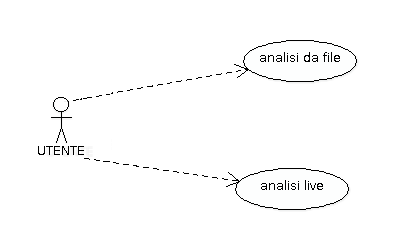
\includegraphics[width=15cm]{usecase1.png}
  \end{center}
  \caption{\label{fig_caso_generale} Casi d'uso}
 \end{figure}\\


\begin{itemize}


\item analisi \textbf{offline} da file: l'utente può far analizzare un file di traffico precedentemente catturato. In gergo
il traffico viene "sniffato", vengono catturati i pacchetti e salvati su file. I programmi maggiormente utilizzati per la cattura sono \textbf{tcpdump} e \textbf{Wireshark}. Il primo esegue da riga di comando e il secondo è una sua interfaccia grafica. Dopo aver catturato il traffico, l'utente esegue l'analisi del file e il sistema riporta 
la presenza o meno di un port scanning da parte di un host remoto e il suo indirizzi ip.

\item analisi \textbf{online} del traffico di rete: l'utente esegue il software che effettua lo "sniffing" live 
del traffico e in modo continuativo la sua analisi. Se viene rilevato uno scanning il sistema esce e riporta la presenza dello scannning e dell'host remoto che l'ha eseguito e il suo indirizzo ip. 

\end{itemize}


\section{Strumenti}

Nel progetto sono stati utilizzati principalmente 2 tool di supporto:

\begin{itemize}

\item \textbf{nmap}: il port scanner open source più utilizzato. Ha moltissime opzioni ed implementa praticamente 
ogni tecnica di port scanning conosciuta.

\item \textbf{wireshark}: uno \emph{sniffer} per l'analisi del traffico. Questo tool l'abbiamo utilizzato per effettuare
il \emph{reverse engineering} di come nmap effettua il port scanning e per salvare il traffico per l'analisi del detector.



\end{itemize}




\section{Scenari}

In questa sezione verranno illustrati i vari possibili scenari in cui l'applicazione vedrà il suo utilizzo. 
In una prima fase l'applicazione verrà installata su uno degli host della propria rete, verrà messa dunque in modalità di sniffing oppure
gli verrà caricato un file di traffico salvato precendentemente. 
Dopo di ciò i casi in cui ci si potrà trovare sono fondamentalmente 2:

\begin{itemize}

\item l'host sul quale è installata l'applicazione non ha servizi attivi, dunque tutte le sue porte sono chiuse.

\item l'host ha attivi alcuni servizi.

\end{itemize}


L'applicazione dunque monitorerà l'host ed "informerà" l'eventuale amministratore di una scansione di porte.\\
Ora dobbiamo vedere quali sono i possibili casi per questa scansione:


\begin{itemize}

\item un host remoto effettua una scansione generale su tutte le porte dell'host.

\item un host remoto scansiona solo un piccolo range di porte, queste possono essere proprio le stesse porte attive sull'host, diciamo 
\emph{n porte} oppure le porte dell'host ed alcune altre, dunque \emph{n + k}.

\end{itemize}


In tutti e due i casi il nostro detector deve avvisare della scansione in corso.




\section{Protocollo Tcp e port scanning}

\begin{figure}[htbp]
\centering
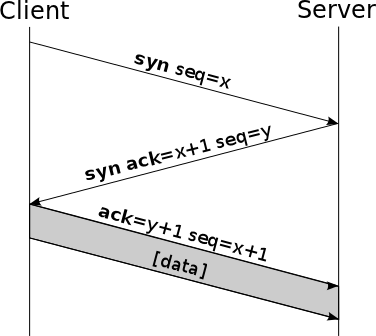
\includegraphics[width=10cm]{tcp.png}
\caption{\label{Protocollo tcp} Protocollo Tcp}
\end{figure}



Nella figura è rappresentata una \emph{connessione tcp} \emph{client-server}. Come si sa, una connessione tcp è formata dal cosiddetto
\emph{Three-way handshake} che può essere riassunto così:

\begin{itemize}

\item il client invia al server un pacchetto con \textbf{flag SYN} impostato ad 1 (attivo) e il campo \emph{sequence number}
inizializzato ad un numero casuale \emph{x}.


\item il server risponde con un pacchetto con \textbf{flag SYN} e \textbf{flag ACK} impostati ad 1, il campo \textbf{sequence number}
impostato ad un valore casuale y e il campo \emph{Acknowledgment number} uguale a \emph{x + 1} 

\item il client risponde al messaggio del server con un pacchetto con \textbf{flag ACK} attivo, il campo \emph{Acknowledgment number} impostato a y + 1 e il campo \textbf{sequence number} uguale a \emph{x + 1}. Ora il client può iniziare
l'invio dei dati al server.


\item se la porta del server sulla quale vuole comunicare il client è chiusa, dopo il primo passaggio il server risponde con un pacchetto con \textbf{flag RST} (reset) attivo e con campo \emph{sequence number} e {Acknowledgment number} come nel secondo passaggio prima. Con il flag rst la connessione tcp viene interrotta e in questo modo il client riconosce che la porta sul server è chiusa e che quindi non può comunicare.


\end{itemize}

\newpage

Uno port scanning non è altro che il tentativo di aprire porte su di un server e riportare quali di queste sono aperte e quali sono
chiuse. Il nostro ports scan detector riesce a riconoscere 2 tipi di port scanning:

\begin{itemize}

\item \textbf{TCP connect scan}: il client completa tutto il \emph{Three-way handshake} su 
ognuna delle porte sottoposte a scanning. E' la tecnica più "rumorosa" perch\`e genera molto traffico ma è anche quella più
affidabile.

\item \textbf{SYN scan}: il client non completa tutte le fasi del protocollo TCP ma si ferma dopo che il server ha risposto con 
il primo pacchetto con \textbf{flag SYN} attivo. Se la porta non fosse aperta infatti il server avrebbe risposto con un pacchetto con 
flag \textbf{RST} attivo. Dunque è corretto ritenere la porta sia aperta.

\end{itemize}




\section{Progettazione}


\begin{figure}[htbp]
\centering
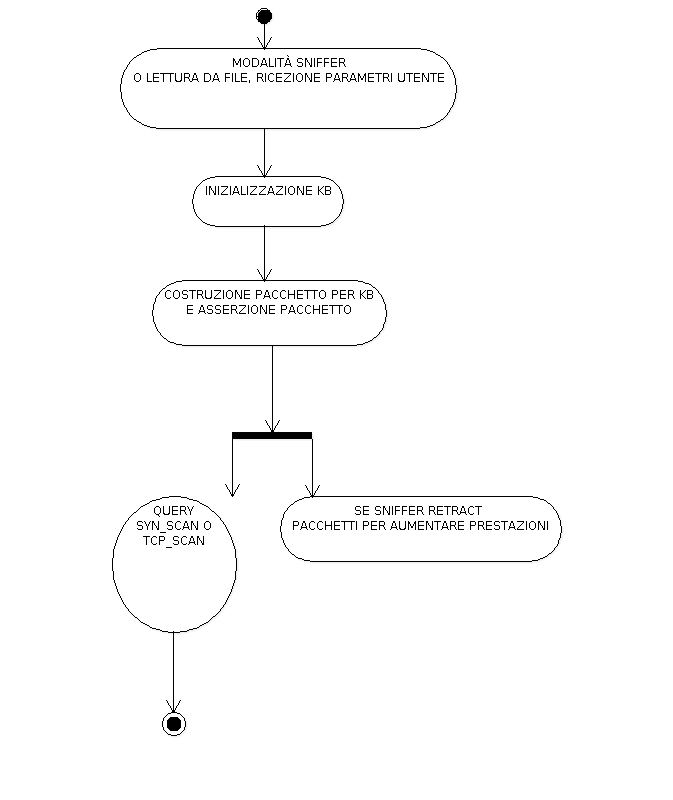
\includegraphics[width=10cm,height=10cm]{attivita.png}
\caption{\label{Diagramma delle attivita} Diagramma delle attivita}
\end{figure}



La figura rappresenta il \emph{diagramma delle attività} dell'intero software. Come si può vedere
all'inizio vengono richiesti i parametri di inizializzazione da parte dell'utente: questi sono del tipo: 



\textbf{kb.pl n\_connections file.pcap sniffer seconds\_retract\_timer}: il primo parametro è la base di conoscenza
scritta in prolog (nelle successive sezioni la descriveremo approfonditamente), il secondo parametro è il numero di connessioni
tcp che devono essere attive affinch\`e venga riconosciuto un port scanning, il terzo parametro invece può rappresentare un 
file di traffico "sniffato" oppure essere la stringa "sniffer": nel primo caso il software effettua l'analisi del file ed inferisce
lo scan o meno, nel secondo caso si avvia in modalità "demone" ed effettua l'analisi \emph{online}. Infine il quarto parametro
rappresenta il numero di secondi da aspettare affinch\`e venga avviato il Thread che effettua il retract dei "fatti" della base di 
conoscenza.





Questo è il diagramma delle classi del progetto:



\begin{figure}[htbp]
\centering
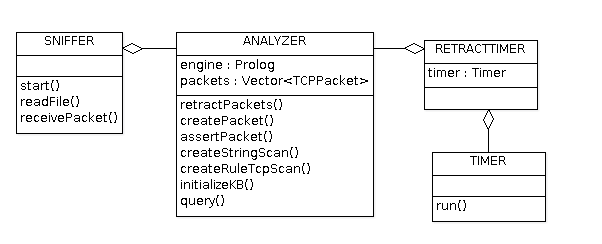
\includegraphics[width=15cm]{classi.png}
\caption{\label{Diagramma delle classi} Diagramma delle classi}
\end{figure}


Descrizione dettagliata delle classi e dei loro metodi:\\


\textbf{SNIFFER}: classe che effettua lo "sniffing" del traffico

\begin{itemize}

\item start(): avvia lo sniffer se in modalità "live"
\item readFile(): legge da file un dump di traffico
\item receivePacket(): ogni volta che lo sniffer riceve un pacchetto viene invocato questo metodo.
Asserisce il pacchetto nella base di conoscenza ed effettua la query per il riconoscimento del port scanning.

\end{itemize}



\textbf{ANALYZER}: classe che si occupa dell'analisi dei pacchetti



\begin{itemize}

\item createPacket(): prende un pacchetto in formato "raw" (jpcap) e costruisce un termine prolog
per la base di conoscenza

\item assertPacket(): asserisce il pacchetto nella base di conoscenza



\item createRuleTcpScan(): crea le regole a partire dal paramentro \textbf{n\_connections} che fornisce l'utente. Ad esempio con 
il parametro uguale a 4 il programma genera la seguente regola: 


\begin{lstlisting}

 tcp_scan(X,Y):- connessione_tcp(X,Y,A1,A2)
,A1\=A2,connessione_tcp(X,Y,A3,A4)
,A3\=A4,connessione_tcp(X,Y,A5,A6),
A5\=A6,A2\=A4,A2\=A6,A4\=A6.
\end{lstlisting}



Il suo significato verrà illustrato meglio nella sezione \ref{Inferenza}.





\item createStringScan(): metodo ausiliario per createRuleTcpScan



\item initializeKB(): inizializza la base di conoscenza con il file prolog ed asserisce la regola 
parametrica dell'utente

\item query(): esegue la query per il port scanning

\item retractPackets(): questo metodo esegue il retract ogni tot secondi (scelti dall'utente) di tutta la base di conoscenza.
E' stato necessario implementare tale metodo per questioni di performance: una base di conoscenza che cresce in modo infinito
porta a prestazioni notevolmente scarse!


\end{itemize}

\textbf{RETRACTIMER}: si occupa di avviare il thread che esegue il retract della base di conoscenza



\section{Tecnologie}

Il progetto è stato realizzato in \emph{Java}. Le librerie che sono state utilizzate sono:


\begin{itemize}

\item jpcap: porting in java della libreria pcap per l'analisi del traffico di rete.

\item tuprolog: libreria java per utilizzare prolog all'interno di codice java. Tra le molte disponibili
è stata utilizzata questa per le migliori prestazioni rispetto alle altre.

\end{itemize}


\section{Inferenza}

In questa sezione viene illustrato il "cuore" dell'applicazione e cioè le regole che definiscono
il motore di inferenza prolog.



\label{Inferenza}
\lstinputlisting{kb.pl}

Il predicato "base" all'interno della KB è \textbf{pacchetto}.
Esso rappresenta un singolo pacchetto nel network
ed è formato da 6 termini:

\begin{itemize}
\item SP: source port, rappresenta la porta sorgente del pacchetto	
\item DP: destination port, rappresenta la porta destinazione del pacchetto
\item syn o rst: rappresentano i flag SYN o RST impostati a 1 del pacchetto. Possono anche non essere presenti.
\item DESTINATION: ip di destinazione
\item SOURCE: ip sorgente
\item le ultime 2 variabili rappresentano rispettivamente l' acknowledgment number e il sequence number
\end{itemize}


Nella base di conoscenza sono presenti anche altre 3 regole: \textbf{connessione\_tcp}, \textbf{connessione\_syn} e \textbf{porta\_chiusa}: 
la prima rappresenta l'inferenza di una connessione tcp tra 2 host su una porta sorgente ed una di destinazione, la seconda
una connessione "syn", cioè che si ferma dopo lo scambio dei primi 2 messaggi tra gli host e la terza la richiesta di un host di una connessione su una porta e la relativa risposta dell'host di destinazione
di porta chiusa.


Come avevamo precedentemente illustrato la regola "principale" della base di conoscenza è quella per il riconoscimento
di uno scanning. Le regole per inferirlo sono 2: una per il riconoscimento di un port scanning tcp e uno per il port scanning
syn. Le regole vengono generate come detto precedentemente utilizzando l'input dell' utente \textbf{n\_connections\_open\_port} e \textbf{n\_connections\_closed\_port} che rappresentano il numero di connessioni tcp che devono essere attive per inferire un port scanning e il numero di porte chiuse che devono essere interrogate.
Le regole ad esempio con richiesta di 4 connessioni aperte e 3 porte chiuse sono generate così:\\


\begin{lstlisting}

 tcp_scan(X,Y):- connessione_tcp(X,Y,A1,A2),A1\=A2,
connessione_tcp(X,Y,A3,A4),
A3\=A4,connessione_tcp(X,Y,A5,A6)
,A5\=A6,connessione_tcp(X,Y,A7,A8),A7\=A8,
A2\=A4,A2\=A6,A2\=A8,A4\=A6,A4\=A8,A6\=A8.

syn_scan(X,Y):- connessione_syn(X,Y,A1,A2),A1\=A2,
connessione_syn(X,Y,A3,A4),A3\=A4
,connessione_syn(X,Y,A5,A6),A5\=A6,
connessione_syn(X,Y,A7,A8),A7\=A8,A2\=A4,A2\=A6,
A2\=A8,A4\=A6,A4\=A8,A6\=A8.
 

tcp_scan(X,Y):- porta_chiusa(X,Y,A1,A2),
A1\=A2,porta_chiusa(X,Y,A3,A4),
A3\=A4,porta_chiusa(X,Y,A5,A6),
A5\=A6,A2\=A4,A2\=A6,A4\=A6.


\end{lstlisting}



Come si può vedere per attivare le regole sono necessarie rispettivamente n connessioni tcp o connessioni syn e n
connessioni di porte chiuse. Sono da notare i vincoli di differenza tra le porte di destinazioni delle varie connessioni.




\section{Compilazione ed esecuzione del progetto}

Per compilare il progetto si utilizza il tool java \textbf{ant}. Un esempio 
di parametri necessari alla compilazione su piattaforma linux:\\

\textbf{sudo ant compile jar"}\\

Questo comando creerà un file \emph{project.jar} all'interno della directory del progetto.\\


Per avviare il progetto invece dare:\\

\textbf{java -jar project.jar opzioni}





\section{Risultati}

Il progetto è stato testato in diverse condizioni di utilizzo:

\begin{itemize}
\item scan delle porte aperte e scan di porte aperte/chiuse
\item nessuna generazione di traffico dell'host sottoposto a scan
\item host sottoposto a scan genera molto traffico
\item l'host viene sottoposto a tcp scan  
\item l'host viene sottoposto a syn scan 

\end{itemize}



In quasi tutti i casi il software si è comportato correttamente riportando lo scan (se i parametri dell'utente erano sufficienti
per riconoscerlo ovviamente). L'unico problema è nello syn scan. In questo particolare scan infatti per essere più "nascosto"
possibile infatti il tool di scanning spesso genera pochissimo traffico e riesce ad eludere il nostro port scanners detector.









\section{Sviluppi futuri}


Nel futuro il progetto potrebbe essere reso un Intrusion Detection System vero e proprio con l'aggiunta
di regole all'interno della sua base di conoscenza e la loro relativa integrazione all'interno del codice
Java. Infine potrebbero essere usati anche approcci di apprendimento automatico per far sì che il progetto
possa migliorare con l'esperienza e dunque limitare al massimo i falsi positivi/negativi. Ad esempio
come dati di apprendimento si possono utilizzare i dati del Dipartimento della difesa americano presente 
a questo indirizzo \href{http://goo.gl/km3RX}{http://goo.gl/km3RX}. 




\end{document}
